\chapter{Project Evaluation}

In this chapter, we evaluate our topic model visualizations against a control interface.
Based on the major pain points discovered in Chapter 3's contextual inquiry, we
focused our user testing on warm-transferred conversations and repeat clients. We
also asked the participants to provide feedback on whether the system helped with
note-taking and which of the four visualizations was most useful.

\section{Users}

For the evaluation, we selected seven volunteers who had been trained as crisis
counselors. These volunteers were assembled from Crisis Text Line and Boston Samaritans,
a local crisis organization that has a texting hotline. Three of the participants worked
for a crisis support center that currently uses the CTL platform to handle clients. The
other four users actively participate in the recruitment of counselors for crisis support
and are familiar with numerous crisis counseling software
systems.

\section{Experiment Protocol}

An evaluation protocol was written with a consent form and instructions for the user.
The experiment consisted of two parts. Part 1 evaluated our visual indexing system
against a control interface, with a focus on completing the three-step counseling
system for warm transfers and repeat clients. Part 2 tested all four visualizations in
the setting of an ongoing conversation as a replacement for note-taking.

\subsection{Part 1}

\begin{figure}[h]
  \centering
    \begin{subfigure}[h]{0.8\textwidth}
      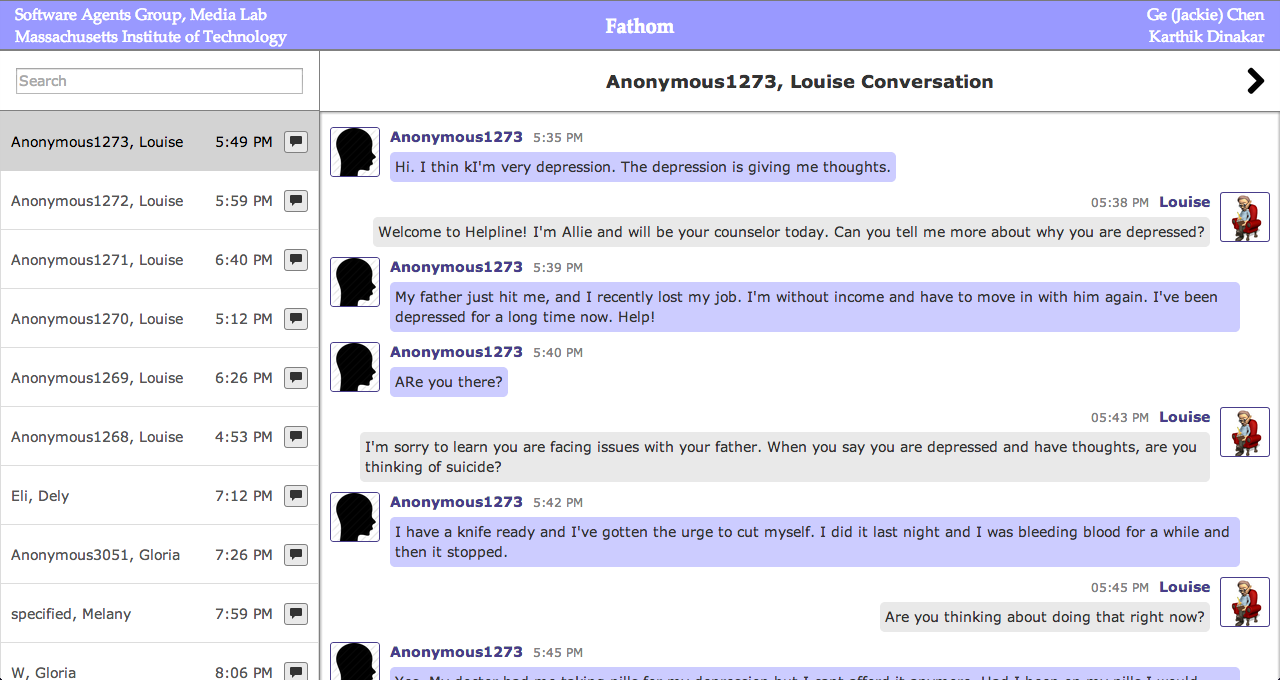
\includegraphics[width=\textwidth]{interface1.png}
      \caption{Interface 1: Control Interface}
      \label{interface1}
      \vspace{3mm}
    \end{subfigure}
    \begin{subfigure}[h]{0.8\textwidth}
      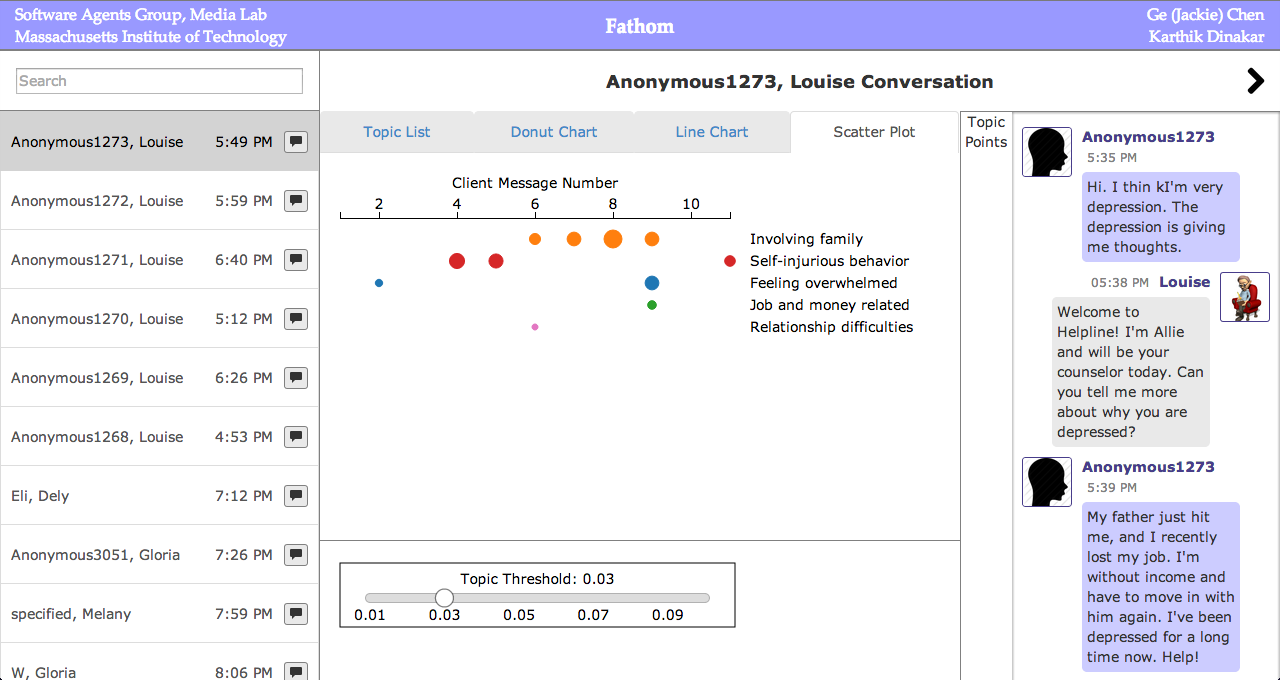
\includegraphics[width=\textwidth]{interface2.png}
      \caption{Interface 2: Scatter Plot Visualization}
      \label{interface2}
    \end{subfigure}
  \caption{Part 1 of the evaluation tested the usefulness of Interface 1 versus Interface
  2 for the completion of the three-step counseling system.}
\end{figure}

In Part 1, the user is asked to imagine him or herself as a counselor at Crisis Text Line.
A fellow overloaded counselor has just given the user a \textit{warm-transferred}
conversation, with which the user must provide a risk assessment, client issues and
emotional state, or an action plan, as part of the three-step counseling system
described in Section 3.1. This is the setup scenario for 12 conversations that the user
must analyze. Six of the conversations are presented using \textbf{Interface 1}, the control
interface shown in Figure~\ref{interface1}, and the other six are displayed with \textbf{Interface 2}, the
scatter plot visualization as seen in Figure~\ref{interface2}. The experimenter shows the user
how to use the scatter plot visualization and set the topic threshold. When using
Interface 2, the user is allowed to use the visualization, the transcript, or a combination
of the two to perform the analysis.

\begin{figure}[h]
  \vspace{3mm}
  \centering
    \fbox{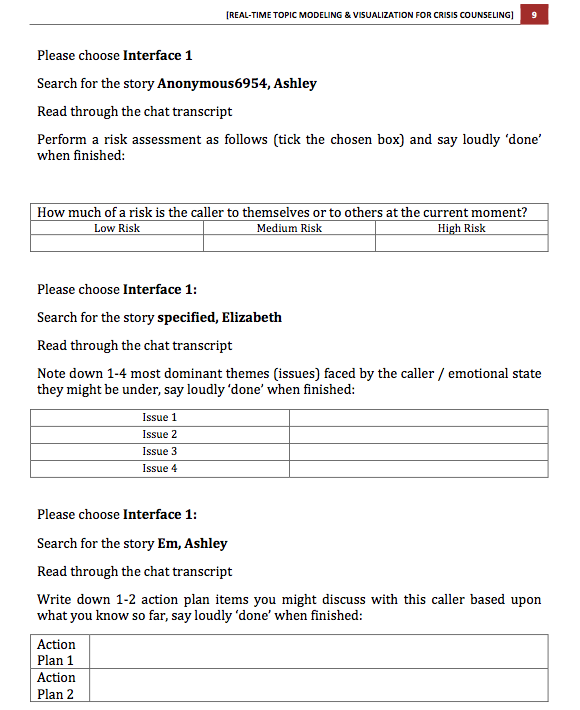
\includegraphics[width=0.75\textwidth]{worksheet.png}}
  \caption{This sample worksheet for the three-step counseling system was given to
  users for Part 1 of the evaluation.}
  \label{worksheet}
\end{figure}

The users are given forms to fill out with their analysis for all 12 conversations,
such as the sample shown in Figure~\ref{worksheet}. After completion, the participants are asked
four questions in Part 1:
\begin{itemize}
  \item \textbf{Q1}: Which interface was useful for a risk assessment of a warm-transferred call,
  and how useful was this interface on a scale of 1 (not useful) to 5 (extremely
  useful)?
  \item \textbf{Q2}: Which interface was useful for eliciting the list of issues and emotional
  state of a warm-transferred call, and how useful was this interface on a scale of
  1 (not useful) to 5 (extremely useful)?
  \item \textbf{Q3}: Which interface was useful for developing an action plan for a
  warm-transferred call, and how useful was this interface on a scale of 1 (not useful) to
  5 (extremely useful)?
  \item \textbf{Q4}: Which interface was useful to get a conversation summary for repeat clients,
  and how useful was this interface on a scale of 1 (not useful) to 5 (extremely
  useful)?
\end{itemize}
In addition to their votes and ratings, users can write open-ended responses to
elaborate on their decisions.

\subsection{Part 2}

In Part 2, the participant is asked to play the role of a live counselor by chatting
in real-time with an experimenter playing a client. This interaction occurs for one
conversation, and the user is allowed to use any of the four topic model
visualizations throughout the conversation. The experimenter demonstrates how to use the
visualizations before evaluation. It is also explained that the visualizations are
updated dynamically with every text received from the client. After the conversation is
complete, the participant must answer the following questions for Part 2:
\begin{itemize}
  \item \textbf{Q5}: How useful was it to view the visualizations in real-time as you were
  chatting with the client, in terms of having to take notes manually, on a scale
  of 1 (not useful) to 5 (extremely useful)?
  \item \textbf{Q6}: Which visualization was the most useful for a visual summary and visual
  indexing, choosing between the Topic List, Donut Chart, Line Chart
  (noncumulative), Line Chart (cumulative), and Scatter Plot?
\end{itemize}
As in Part 1, the users are allowed to provide additional feedback in the form of
open-ended responses.

\section{Results}

\begin{table}[h]
  \centering
  \begin{tabular}{| c | c c | c c |}
    \hline
    Question Number & \multicolumn{2}{|c|}{Interface 1} & \multicolumn{2}{|c|}{Interface 2} \\
    \hline \hline
    & Votes & Average Rating & Votes & Average Rating \\
    \hline
    Q1 & 71.38\% & 2.6 & 28.57\% & 3.5 \\
    Q2 & 14.28\% & 3 & 85.71\% & 3.9 \\
    Q3 & 57.14\% & 3 & 42.85\% & 3.3 \\
    Q4 & 0\% & N/A & 100\% & 4.42 \\
    \hline
  \end{tabular}
  \caption{This table summarizes the answers given by participants to questions 1-4
  in Part 1. Users preferred the control interface for assessing risk and developing an
  action plan, but they favored the scatter plot visualization even more for eliciting
  issues and summarizing conversations for repeat clients.}
  \label{tab:results}
\end{table}

The results for Part 1 are shown in Table~\ref{tab:results}. Users found the control interface
to be more useful for assessing risk and developing an action plan. In the feedback,
most participants said they preferred to read specific parts of the transcript at the
beginning for risk assessment. However, questions two and four presented completely
different outcomes. Almost 86 percent of users felt that the scatter plot visualization
was more useful for eliciting client issues and emotional state, while all participants
favored it as a summary for repeat clients. These preferences for our system also
had the highest average ratings of the group. Even when users preferred Interface 1,
Interface 2 produced higher average ratings across the board.

In Part 2, responses to question \textbf{Q5} produced an average rating of 4. This result
illustrates that the topic model visualizations are a worthwhile replacement or
complement to manual note-taking. For question \textbf{Q6}, four users said that the Scatter
Plot was the most effective visualization for visual indexing, two preferred the Topic
List for a visual summary, and one found the Line Chart (noncumulative) to be most
useful. These results agree with our hypotheses that visual indexing is a valuable
feature of our system, and that counselors care more about the topics and their relative
dominance than the specific proportions.

Finally, the open-ended evaluations given by the users were constructive for future
ideas. Participants expressed much enthusiasm for this work, but they were also eager
for more features. One common piece of feedback was to visualize counselor notes in
addition to conversation summaries. Three of the users also believed that it would
be beneficial to highlight certain topics, such as suicide ideation or risk, no matter
what their topic model proportions are.
